\subsection{Data}

We used a data set following migration experiences collected by
\citet[][]{Kreienkamp2022b}. The data set consists of three studies that
followed migrants who had recently arrived in the Netherlands in their
daily interactions with the Dutch majority group members. After a
general migration-focused pre-questionnaire, participants were invited
twice per day to report on their (potential) interactions with majority
group members for at least 30 days. The short ESM surveys were sent out
at around lunch (12pm) and dinner time (7pm). After the 30 day study
period participants filled in a post-questionnaire that mirrored the
pre-questionnaire. Participants received either monetary compensation or
partial course credits based on the number of surveys they completed.
For our empirical example we focus on the variables that were collected
during the ESM surveys and were available in all three studies. Full
methodological details are available in \citet[][]{Kreienkamp2022b}.

\subsubsection{Sample}

The original studies included 207 participants (\(N_{S1}=\) 23,
\(N_{S2}=\) 113, \(N_{S3}=\) 71) with a total of 10,297 measurements.
The studies differed substantially in the maximum length of
participation (\(\text{max}(t_{S1})=\) 63, \(\text{max}(t_{S2})=\) 69,
\(\text{max}(t_{S3})=\) 155). This was likely due to the option to
continue participation without compensation in the later two studies. To
make the three studies comparable in participation and time frames, we
iteratively removed all measurement occasions and participants that had
more than 45\% missingness
\citep[which was in line with the general rcecommendation for data that might still need to rely on imputations for later model testing][]{Madley-Dowd2019}.
This procedure let to a final sample of 157 participants, who jointly
produced 8,132 measurements. Importantly, both the participant
repsonse-patterns and the time frame were now a lot more comparable
(\(\text{max}(t_{S1})=\) 61, \(\text{max}(t_{S2})=\) 60,
\(\text{max}(t_{S3})=\) 67). For a full overview of the data reduction
procedure and study-specific exclusions see Online Supplemental Material
A.

\subsubsection{Variables}

We included 12 variables that were available across all three studies
and captured information about the participant's interactions, as well
as cognitive-, emotional-, and motivational self in relationship with
the majority group. We chose these two aspects in particular because (1)
the interaction-specific information exemplified the structural
missingness issue of modern ESM data and (2) the motivational,
emotional, and cognitive experience offered a diverse conceptualization
of migration experience (beyond behavioral measurements) that is
becoming more common in the literature \citep[][]{Kreienkamp2022d}. Full
methodological details are available in Online Supplemental Material A,
but basic item information, descriptives, and correlations are also
available in \tblref{tab:descrLong}.

\begin{sidewaystable*}[!hbtp]
\centering

\caption{\label{tab:descrLong}Correlation Table and Descriptive Statistics}
\centering
\resizebox{\linewidth}{!}{
\begin{tabular}[t]{lcccccccccccc}
\toprule
  & \makecell{Int: \\ Accidental} & \makecell{Int: \\ Voluntary} & \makecell{Int: \\ Cooperative} & \makecell{Int: \\ Representative} & \makecell{Int: \\ Meaningful} & \makecell{Int: \\ Quality} & Core Need & \makecell{Core Need \\ Due to Partner} & \makecell{Attitude \\ Partner} & \makecell{Daytime \\ Core Need} & \makecell{Outgroup \\ Attitude} & Well-being\\
\midrule
\addlinespace[0.3em]
\multicolumn{13}{l}{\textbf{Correlations}}\\
\hspace{1em}Int: Accidental &  & -0.20 & -0.21* & 0.07 & -0.10 & -0.13 & -0.39*** & -0.26* & -0.05 & -0.28** & -0.03 & 0.12\\
\hspace{1em}Int: Voluntary & -0.14*** &  & 0.63*** & -0.04 & 0.12 & 0.44*** & 0.19 & 0.16 & 0.42*** & 0.10 & 0.25** & -0.05\\
\hspace{1em}Int: Cooperative & -0.14*** & 0.32*** &  & 0.19 & 0.38*** & 0.68*** & 0.42*** & 0.53*** & 0.47*** & 0.24* & 0.28** & -0.08\\
\hspace{1em}Int: Representative & 0.28*** & 0.39*** & -0.11*** &  & 0.10 & 0.13 & -0.09 & -0.03 & 0.14 & -0.02 & 0.43*** & -0.07\\
\hspace{1em}Int: Meaningful & 0.01 & 0.06** & 0.21*** & 0.30*** &  & 0.66*** & 0.11 & 0.20 & 0.44*** & 0.10 & 0.01 & -0.03\\
\hspace{1em}Int: Quality & 0.07** & 0.44*** & 0.33*** & 0.04 & 0.16*** &  & 0.42*** & 0.34*** & 0.65*** & 0.23* & 0.25* & 0.07\\
\hspace{1em}Core Need & 0.12*** & -0.07** & 0.08*** & 0.41*** & 0.02 & -0.02 &  & 0.65*** & 0.11 & 0.64*** & 0.15 & 0.30**\\
\hspace{1em}Core Need Due to Partner & -0.18*** & 0.18*** & 0.20*** & 0.58*** & 0.15*** & 0.15*** & 0.19*** &  & 0.14 & 0.53*** & 0.13 & 0.07\\
\hspace{1em}Attitude Partner & 0.21*** & 0.27*** & 0.32*** & 0.24*** & 0.17*** & 0.17*** & 0.22*** & 0.16*** &  & -0.09 & 0.57*** & 0.08\\
\hspace{1em}Daytime Core Need & 0.29*** & 0.10*** & 0.53*** & 0.26*** & 0.15*** & 0.14*** & 0.37*** & 0.17*** & 0.33*** &  & 0.07 & 0.17\\
\hspace{1em}Outgroup Attitude & 0.01 & 0.18*** & -0.04 & -0.06* & 0.14*** & 0.20*** & 0.09*** & -0.03 & 0.16*** & 0.26*** &  & 0.21*\\
\hspace{1em}Well-being & -0.09*** & 0.33*** & 0.30*** & 0.11*** & 0.09*** & 0.31*** & -0.06** & 0.23*** & 0.14*** & 0.20*** & 0.24*** & \\
\addlinespace[0.3em]
\multicolumn{13}{l}{\textbf{Descriptives}}\\
\hspace{1em}Grand Mean & 39.10 & 80.08 & 79.55 & 64.65 & 61.16 & 79.85 & 85.42 & 78.52 & 80.59 & 76.48 & 66.84 & 49.64\\
\hspace{1em}Between SD & 31.14 & 20.61 & 18.41 & 21.12 & 24.62 & 17.05 & 16.01 & 21.53 & 16.33 & 21.63 & 18.54 & 31.95\\
\hspace{1em}Within SD & 28.72 & 19.27 & 17.43 & 19.92 & 22.32 & 16.37 & 18.63 & 20.02 & 15.81 & 22.26 & 9.45 & 25.72\\
\hspace{1em}ICC(1) & 0.21 & 0.29 & 0.27 & 0.35 & 0.31 & 0.25 & 0.18 & 0.26 & 0.25 & 0.20 & 0.77 & 0.52\\
\hspace{1em}ICC(2) & 0.90 & 0.93 & 0.93 & 0.89 & 0.94 & 0.92 & 0.91 & 0.92 & 0.91 & 0.92 & 0.99 & 0.98\\
\bottomrule
\multicolumn{13}{l}{\rule{0pt}{1em}\textit{Note: }}\\
\multicolumn{13}{l}{\rule{0pt}{1em}Upper triangle: Between-person correlations;}\\
\multicolumn{13}{l}{\rule{0pt}{1em}Lower triangle: Within-person correlations;}\\
\multicolumn{13}{l}{\rule{0pt}{1em}*** p < .001, ** p < .01,  * p < .05}\\
\end{tabular}}
\end{sidewaystable*}


\subsection{Analysis and Results}

To perform the main analysis on our selected variables, we showcase the
extract--reduce--cluster--evaluate steps in sequential order. For each
of the steps fully reproducible and annotated code is available in
Online Supplemental A as well as in the accompanying OSF- and GitHub
repositories (REF).

\subsubsection{Feature extraction}

For the features, we selected and extracted one of each of the features
proposed in \tblref{tab:esmFeatures}. We particularly chose the more
robust median and median absolute deviation (MAD) for central tendency
and variability. Within the variability structure, we chose the slightly
more intuitive mean absolute change (MAC) for stability and stayed with
the common lag--1 autocorrelation for inertia. For the trend summaries,
we chose the overall linear regression slope to describe the linear
trend and we summarized the nonlinear trend with the estimated degrees
of freedom of an empty GAM spline model (edf) --- the edf summarizes the
\textit{wiggliness} of the spline trend line. We chose these features in
particular because we consider them to be the most broadly applicable
features. We also extracted the participant's number of completed ESM
measurements to ensure that the clusters are comparable in that regard.
We provide an R-function that automatically extracts and prepares a
large selection of the time series feature operationalizations presented
in \tblref{tab:esmFeatures} in our GitHub repository (see the
\texttt{featureExtractor} function).

For the central tendency: \(Median\) where \(X_{ij}\) is the an ordered
list of values from the time series of variable \(j\) for participant
\(i\).

\begin{equation}
  Median(X_{ij}) = \left\{ 
    \begin{array}{ll}
      X \left[ \frac{n+1}{2} \right] & \text{if $n$ is odd} \\
      \frac{X \left[ \frac{n}{2} \right] + X \left[ \frac{n}{2} +1 \right]}{2} & \text{if $n$ is even}
    \end{array}
\end{equation}

\begin{equation}
  Median(X_{ij}) = 
    \begin{cases}
      X \left[ \frac{n+1}{2} \right] & \text{if $n$ is odd} \\
      \frac{X \left[ \frac{n}{2} \right] + X \left[ \frac{n}{2} +1 \right]}{2} & \text{if $n$ is even}
    \end{cases}
\end{equation}

For distribution

After the feature extraction, we found that about 1.40\% of the
extracted features are missing across the 72 features per participant.
This might, for example, happen if participants do not have two
subsequent measurements with outgroup interactions, so that an
autocorrelation with lag-1 cannot be calculated for the contact-specific
variables. The small number of missing values indicates that the
feature-based approach indeed largely avoids the structural missingness
issue. The few missing values can, however, be an issue for some feature
reduction or feature clustering algorithms. We, thus, impute the missing
feature values with a single predictive mean matching imputation using
the MICE library.

\subsubsection{Feature reduction}

For the feature reduction, we chose the common
\textit{principal component analysis} (PCA). Some of the more
tailor-made feature selection algorithms can be more accurate in
reducing the feature dimensionality and might retain feature importance
information more directly, depending on the specific data structure.
However, PCAs have the distinct benefit that they are well-established
within the psychometric literature and can broadly be applied to a wide
variety of studies in an automatize manner. As our aim is to present a
general illustration that can also be adopted for more general data
descriptive uses, we present the workflow using a PCA here but we
encourage users to consider more specialized methods as well.

To use the principal component analysis with our extracted time series
features, we first standardize all features across participants to
ensure that all features are weighted equally. We then enter all 72
features into the analysis. The PCA will use linear transformations in
such a way that the first component captures the most possible variance
of the original data (e.g., by finding a vector that maximizes the sum
of squared distances). The following components will then use the same
method to iteratively explain the most of the remaining variance while
also ensuring that the components are linearly uncorrelated. In
practice, this meant that the PCA decomposed the 72 features into 72
principal components but now (because of the uncorrelated linear
transformations) the first few principal components will capture a
majority of the variance. We can then decide how much information (i.e.,
variance) we are willing to sacrifice for a reduced dimensionality. A
common rule of thumb is to use the principal components that jointly
explain 70--90\% of the original variance (i.e., cumulative percentage
explained variance). For our illustration we select the first 27
principal components that explain 80\% of the variance in the original
72 features (reducing the dimensionality by 62.50\%). For the extracted
principal components we save the 27 PC-scores for each participant
(i.e., the participants' coordinates in the reduced dimensional space).

We would like to comment on two practical matters when using principal
components --- the amount of dimensionality reduction and the
interpretation of the principal components. As for the expected
dimensionality reduction, given its methodology, PCAs tend to `work
better' at reducing dimensions with (highly) correlated variables. Thus,
with a set of very homogeneous variables and features users will need
less principal components to explain a large amount of variance, while a
more diverse set of variables and features will tend to require more
principal components to capture the same amount of variance. Our 27
principal components are still a relatively high number of variables but
this is not surprising as we chose a diverse conceptualization and a
diverse set of time series features. As for the interpretability, PCA
allows users to extract information on the meaning of the principal
components. In particular, because the principal components are linear
combination of original features, users can extract the relative
importance of each feature for the extracted principal components (i.e.,
the eigenvectors). While this can be useful in understanding the
variance in the original data or help with manual feature selection, we
use the PCA purely to reduce the dimensionality for the clustering step.
Instead of relying on the principal components, we use the original
features of interest to interpret the later extracted clusters. We
particularly advocate for such an approach if the original features were
chosen for their psychological meaning in understanding the time series
and broader phenomenon of interest.

\subsubsection{Feature clustering}

For our illustration of the feature clustering procedure, we use the
generalizable and efficient centroid-based k-means clustering. The
procedure needs the user to make a selection on the optimal number of
clusters in order to run the main algorithm. We use the Elbow and the
Silhouette method, which both suggest two clusters to be the optimal
solution (see Supplemental Material A). We then entered the
participants' PC-scores into the k-means algorithm. We used the
recommended Hartigan and Wong algorithm \citep{hartigan1979} with 100
random initial centroid positions to avoid convergence to a sub-optimal
solution (i.e., local minima). The k-means analysis assigned 80
participants to cluster 1 and 76 participants to cluster 2.

In order to interpret the two clusters, we compare the two clusters in
their features as well as in their raw time series. We first inspect the
clusters with a focus on the included variables (see
\fgrref[A]{fig:clusterFeatVar}). We (1) see that for some variables the
features are generally stronger in separating the clusters (e.g., `how
cooperative an interaction was' compared to `attitudes towards the
Dutch'). Additionally, we see that (2) within the variables some
features are better at distinguishing clusters (e.g., median of
well-being vs.~MAC of well-being).We then inspect the clusters with a
focus on the features (see \fgrref[B]{fig:clusterFeatVar}). While this
is the same data as for the variable focus, we can see more clearly that
some features are better at distinguishing the clusters across variables
(e.g., mean and median compared to auto correlations). This offers some
information on which features were are most important in understanding
the two extracted groups.

\begin{figure}[!ht] %hbtp
  \caption{Cluster Group Comparisons based on Features and Variables}
  \label{fig:clusterFeatVar}
  \centering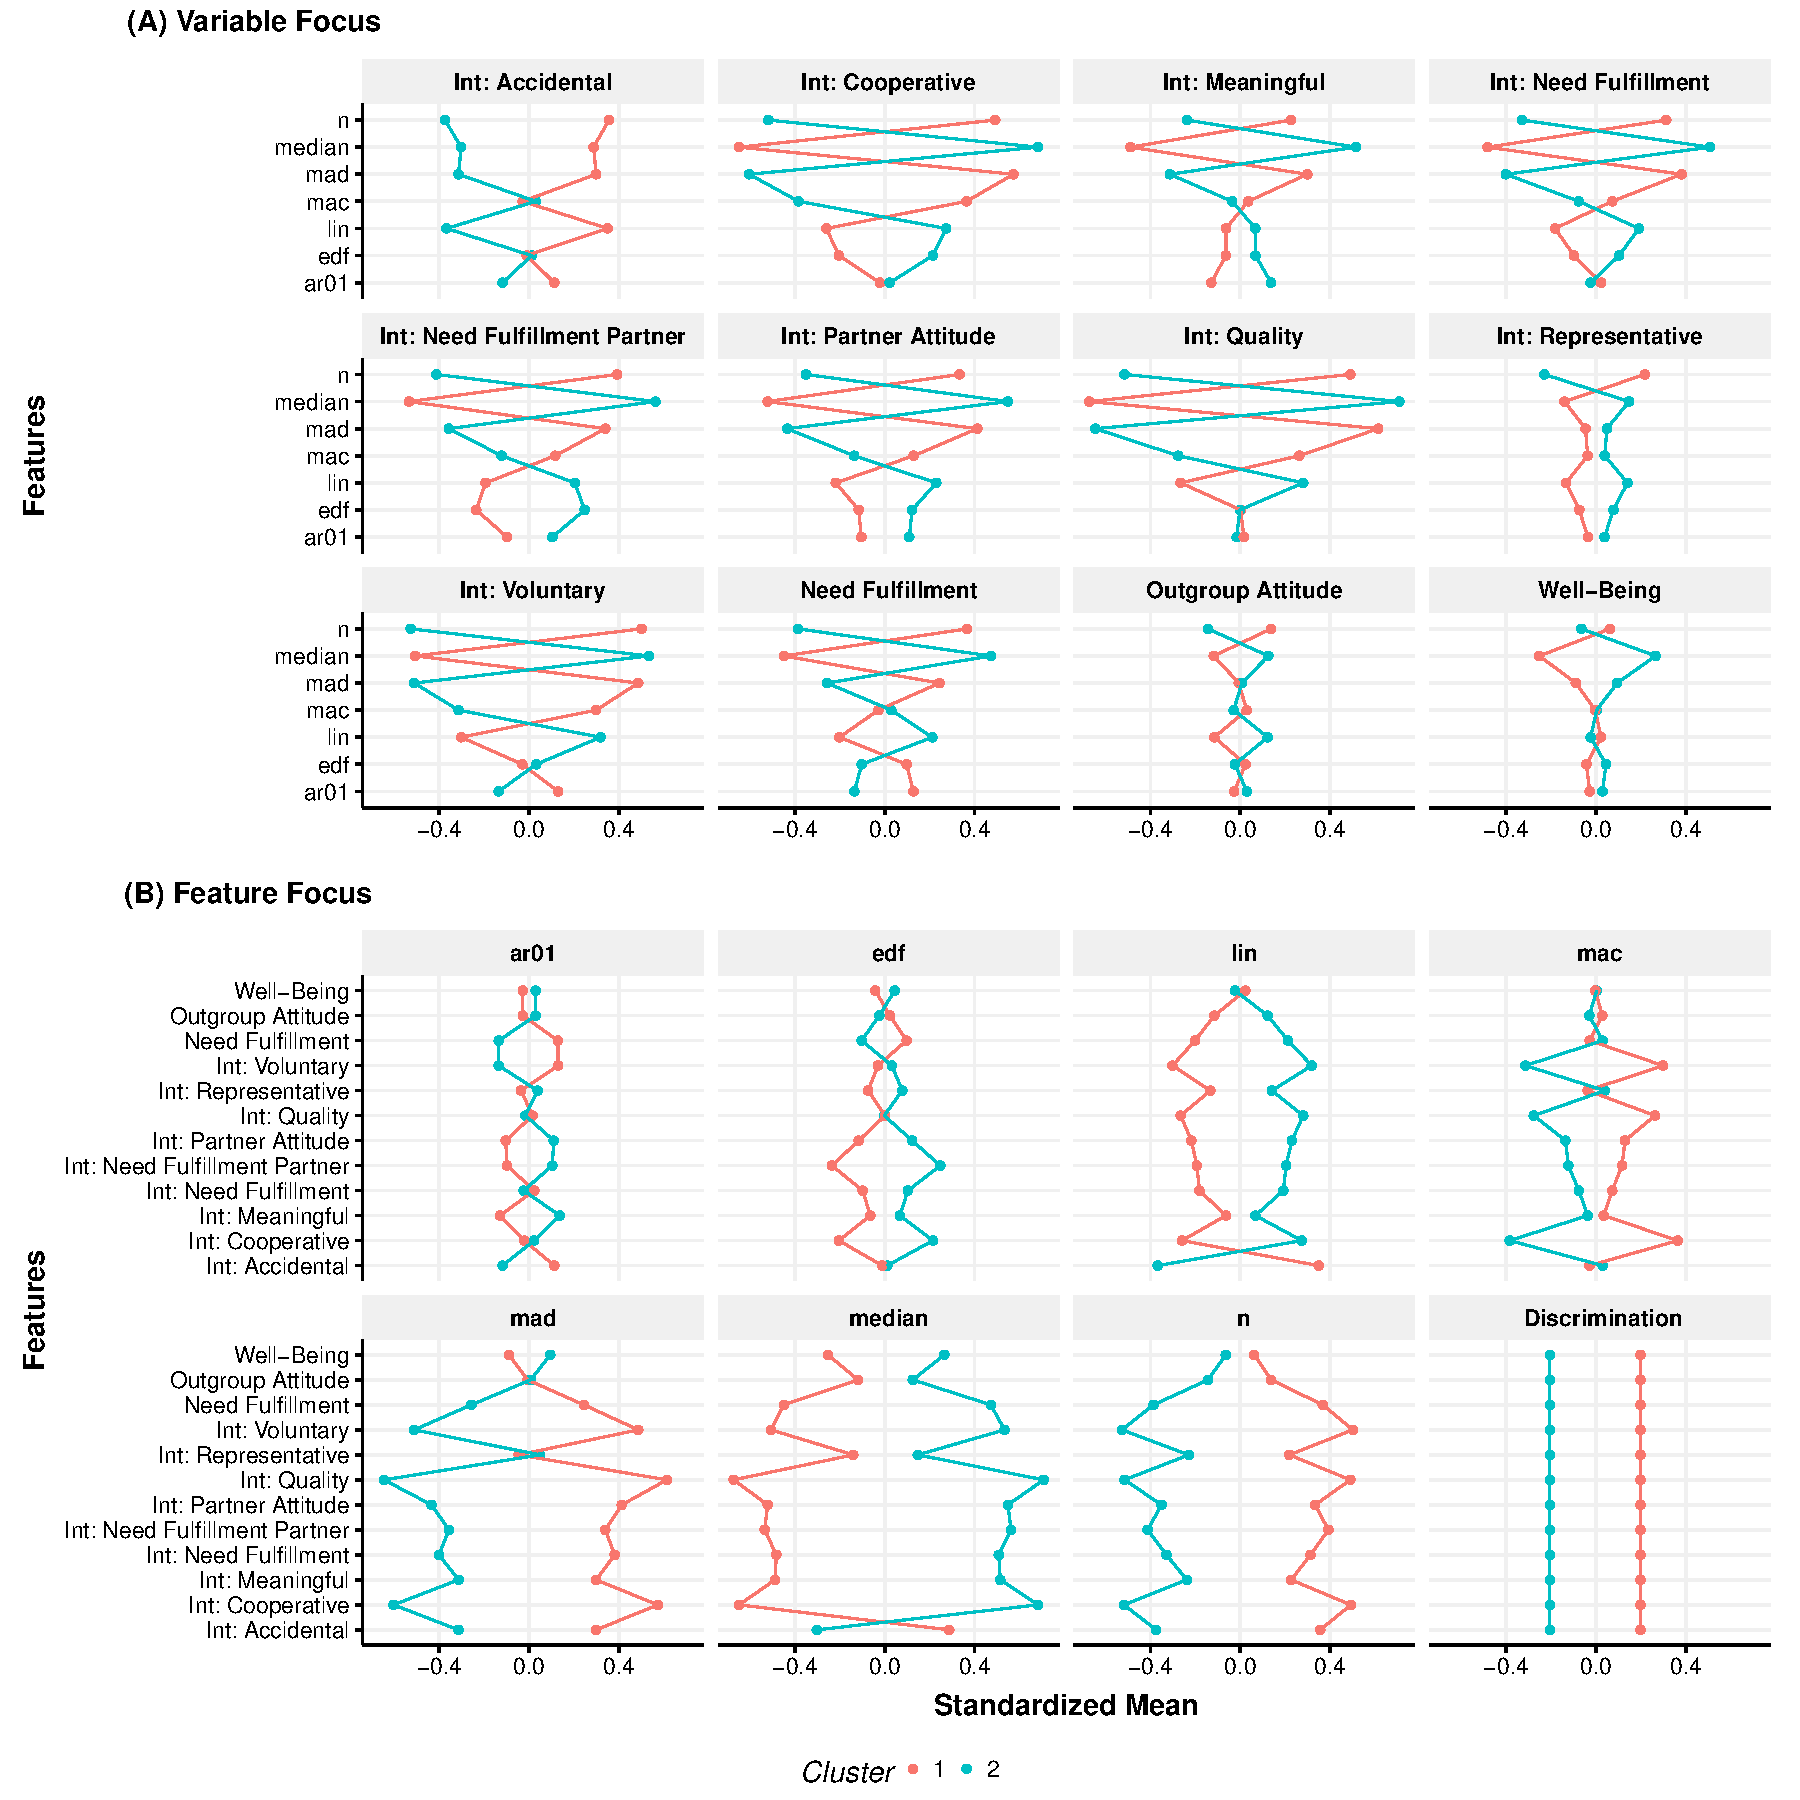
\includegraphics[width=\textwidth]{figures/clusterFeatVarComb.pdf}
  \caption*{Note: \\
  Within the "(B) Feature Focus" subplot, the 'n' and 'Discrimination' comparison variables were not part of the original time series clustering.}
\end{figure}

We can then combine the two focus approaches to assess the developments
between the two groups more holistically (see \fgrref{fig:clusterTs}).
Immediately striking are the mean differences, where participants in the
second cluster had more meaningful and fulfilling outgroup interactions
also consistently reported more voluntary and cooperative interactions
but less accidental and involuntary interactions. The same cluster also
reported an increase in need fulfilling interaction over the 30 day
period and an increase in interactions that were representative of the
outgroup. Whereas the other cluster showed a decrease in voluntary,
cooperative, and positive interactions over the 30 days. This
`deterioration' cluster also saw a decrease in general need fulfillment
and experienced well-being over the 30 days (see
\fgrref[B]{fig:clusterTs}). We also see that while interaction
representativeness, outgroup attitudes, well-being are relatively stable
for both clusters, the deteriorating cluster also showed substantially
higher variablity and instability over time (also see
\fgrref[A]{fig:clusterTs}).

We can also assess the clusters across any other person-level variable.
This out-of-feature comparison allows us to check for data artifacts, as
well as check whether the developmental clusters are associated with
important social markers and individual differences. To illustrate
artifact checks, we added the number of measurements into the comparison
and find that the participants in the detereoration cluster on average
completed more ESM surveys and reported on more intergroup interactions
than the cluster with the more positive interactions (see
\fgrref[B]{fig:clusterTs}). While this difference could indicate that
the clusters might not entirely be comparable in the response patterns,
we can find some relief in our data exclusion procedures during which we
ensured that the general time frame and completion rates were not too
dissimilar. To illustrate the utility of individual differences, we
compare the two samples in terms of the participants' self-reported
discrimination experiences in the Netherlands (measured during the
post-measurement). \fgrref[B]{fig:clusterTs} illustrates that
participants in the deteriorating cluster reported substantially higher
levels of everyday discrimination. Thus, both intensive longitudinal and
cross-sectional variables that were not included in the original
clustering step can be used to explore and understand the cluster
differences in more detail.

\begin{figure}[!ht] %hbtp
  \caption{Cluster Group Comparisons over time}
  \label{fig:clusterTs}
  \centering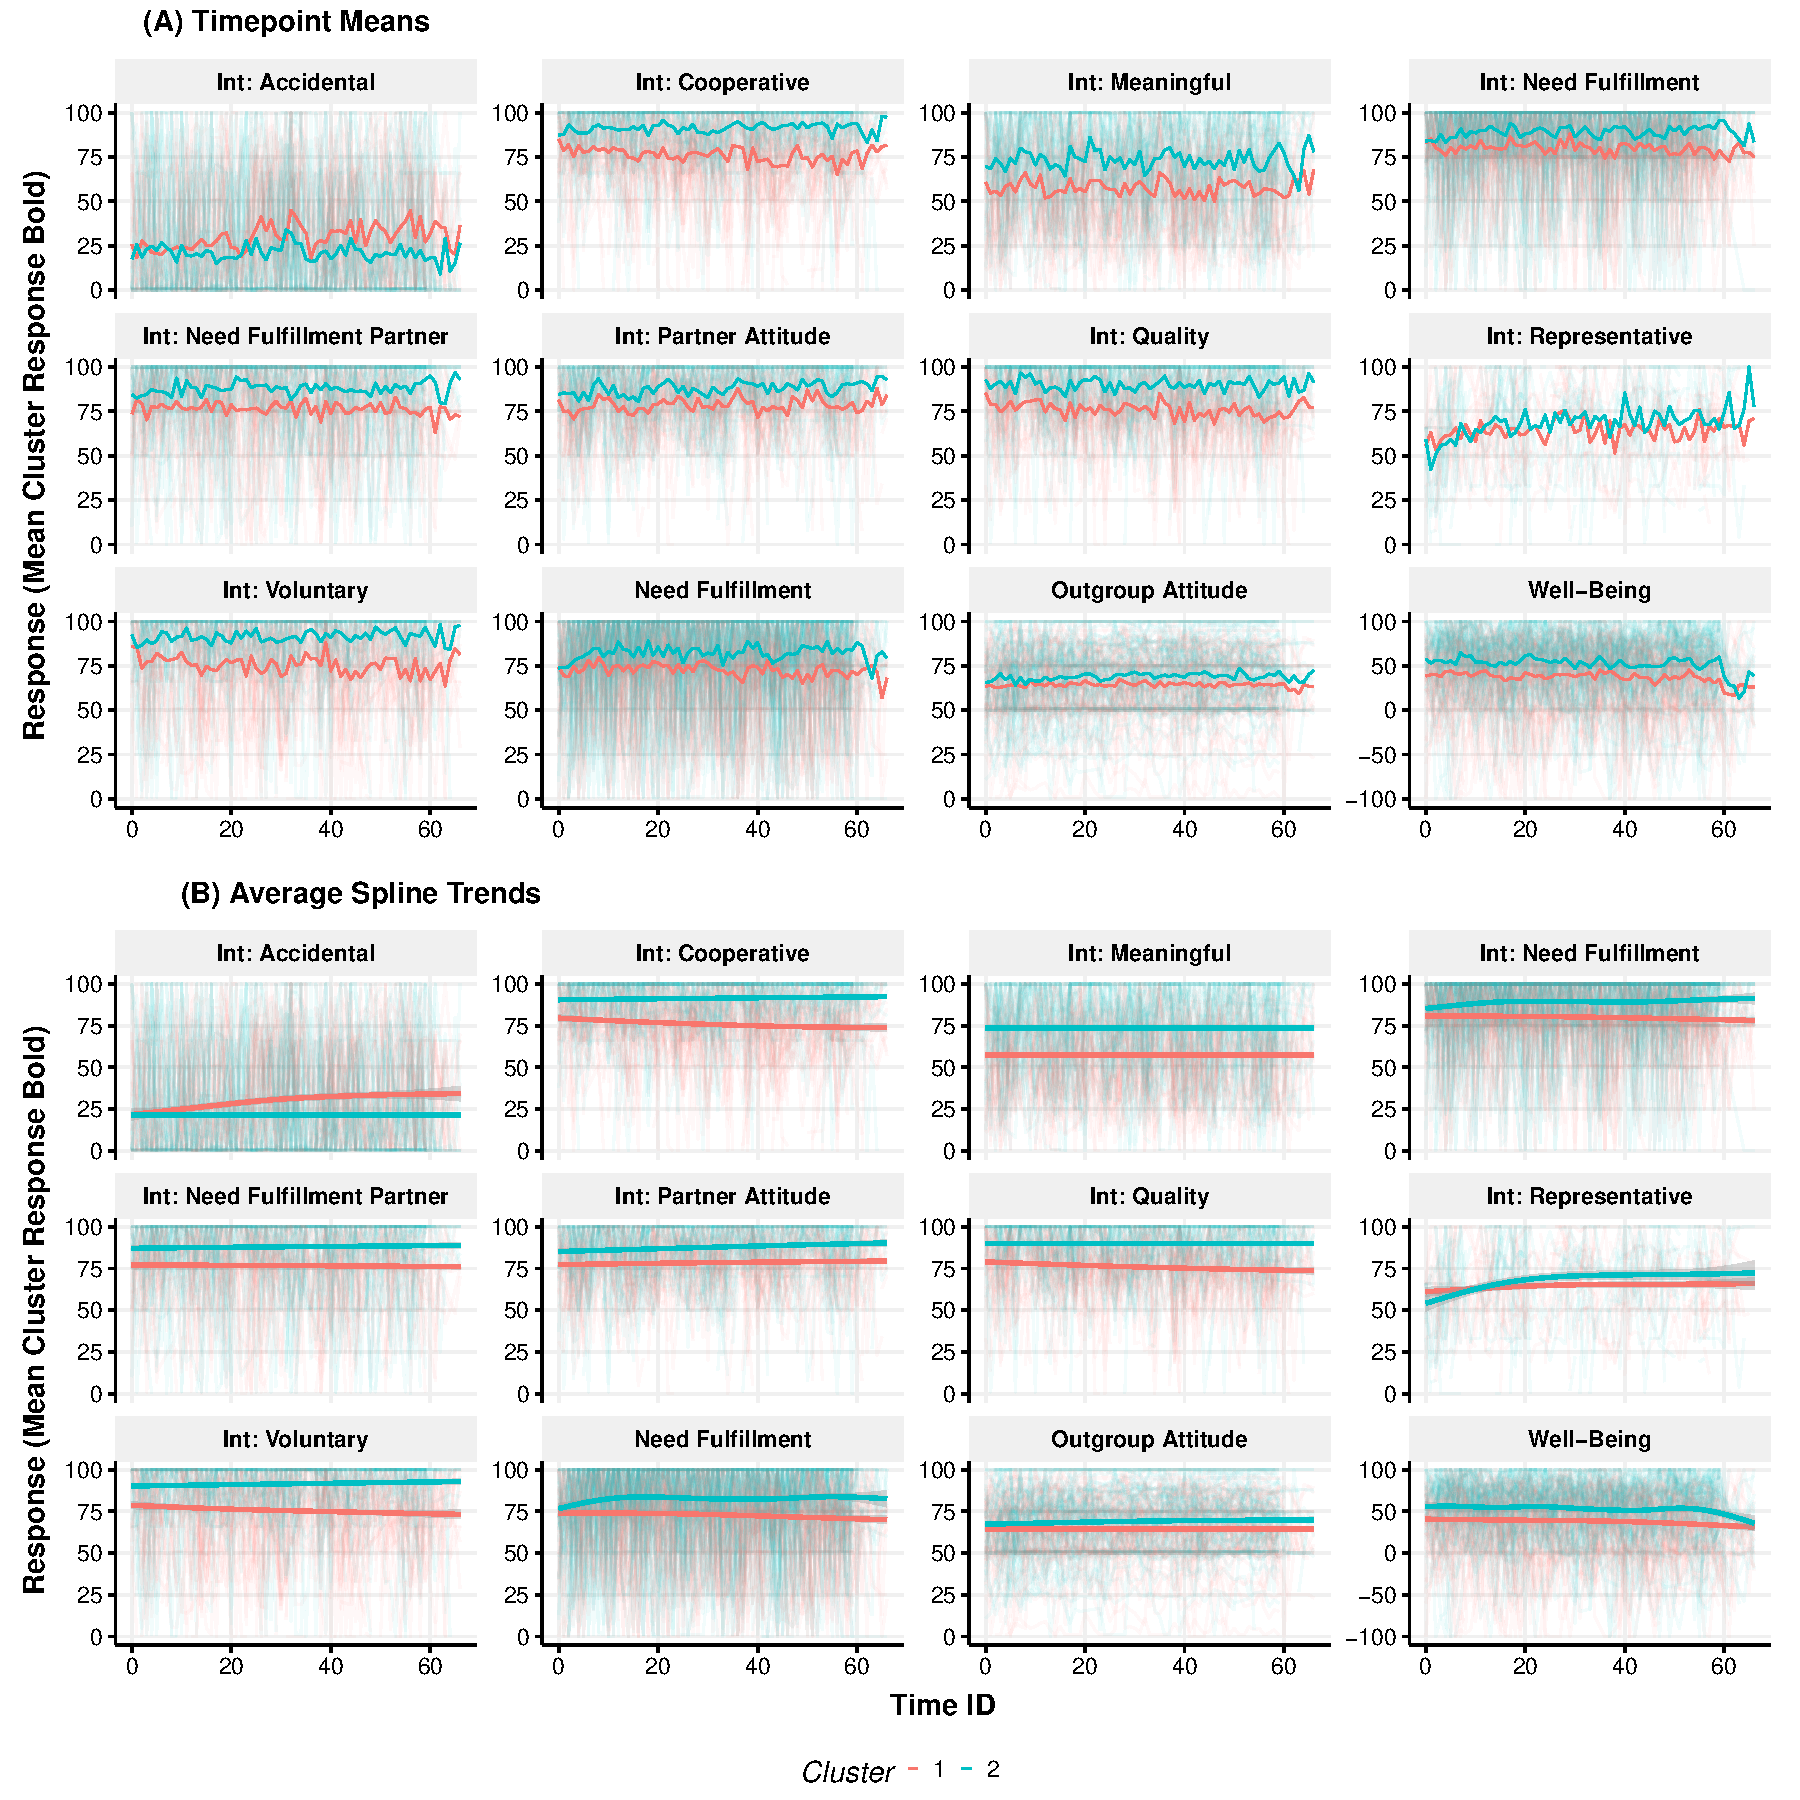
\includegraphics[width=\textwidth]{figures/clusterTsComb.pdf}
  \caption*{Note: \\
  Subplot (A) displays the variable cluster means at every measurement occasion. Subplot (B) shows the GAM spline for each cluster across the measurement occasions.}
\end{figure}
